\chapter{Introduction}
\label{cap:introduction}

\section{The Company}
\href{https://www.221e.com/about-us}{221e S.r.l.}\footcite{site:221e} is an innovative startup established in 2012 in Italy. It has business units in Padova, Treviso, and Bergamo. The company leverages microelectronics, sensors and control algorithms to develop miniaturized wireless embedded systems.

221e operates under a dual-layer business model and offers:
\begin{enumerate}
    \item OEM (Original Equipment Manufacturer) services to third-party clients needing a technology partner for product development. This involves R\&D contracts followed by commercial agreements for the supply of engineered systems.
    \item Finished products, both general-purpose multi-sensor hardware platforms and a software for controlling the systems. 
\end{enumerate}

Targeting the Wearable Devices market and, more in general, the Internet of Things (IoT) industry, 221e capitalizes on the limitless applications within these fields. 

\begin{figure}[htbp]
    \centering
    
\includegraphics[height=2cm]{221e_logo.png}
    \caption{221e's logo}
\end{figure}

\begin{figure}[htbp]
    \centering
    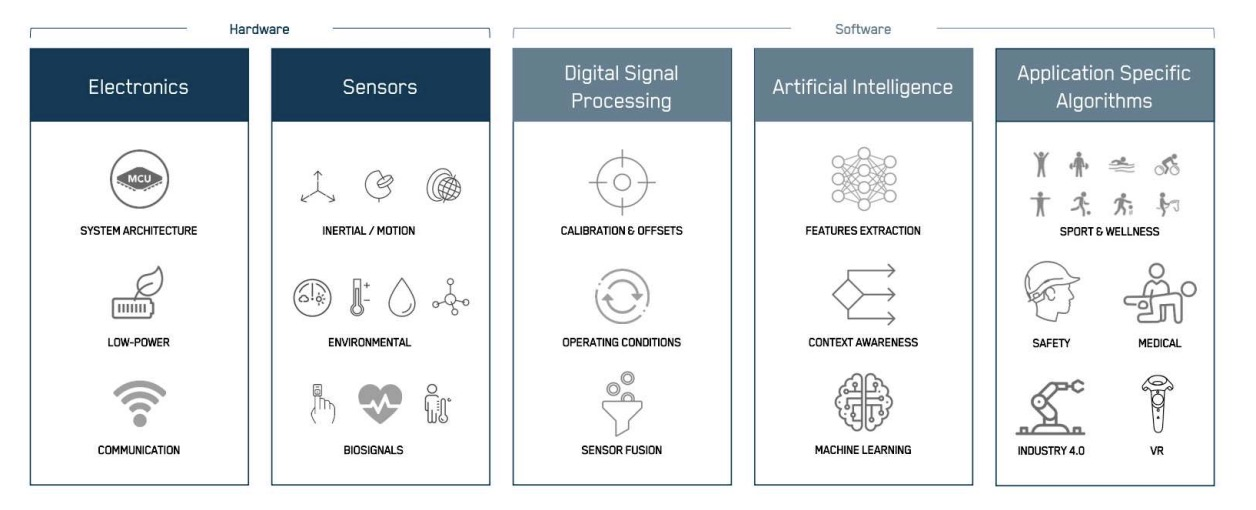
\includegraphics[width=\textwidth]{221e_applications.png}
    \caption{221e's technology echosystem}
\end{figure}


\newpage
\section{Objectives and requirements}
\label{sec:objectives-and-requirements}

The idea of the project is to create a cloud-agnostic\footnote{Cloud Agnostic: Able to be deployed on every cloud provider effortlessly} architecture for a network of heterogeneous \textbf{IoT devices}\footnote{IoT Devices: Devices connected to the internet and equipped with a set of sensors. Each device sends data to a broker using an appropriate protocol.}. The architecture needs to provide a way to ingest, to store and to analyze data ingested from multiple sensors. The architecture must also be designed to be able to scale horizontally\footnote{Horizontal scaling: capability of adding more machines or nodes to a system to handle an increase in workload} and vertically\footnote{Verical scaling: capability of increasing the capacity of a single machine or server by adding more resources such as CPU, RAM, or storage.}.

\subsection{Cloud Infrastructure}
The architecture needs to ingest, store and process large amounts of IoT data leveraging the power of cloud services. The final product to be developed is an architecture that can be deployed on any cloud provider. The main advantage of the architecture being cloud-agnostic is that since it can be deployed on any cloud provider, virtually without any modification each customer is able to choose the cloud provider that best fits his needs.
The providers taken into account to develop the architecture during this project are the following: \href{https://www.arubacloud.com/}{Aruba Cloud}\footcite{site:aruba-cloud}, \href{https://aws.amazon.com/it/}{Amazon Web Services}\footcite{site:aws} and \href{https://azure.microsoft.com/it-it/}{Microsoft Azure}\footcite{site:azure}. 
AWS\footnote{AWS: Amazon Web Services} and Microsoft Azure were chosen because of already developed experience of the company, and me. Aruba Cloud instead has been used because of a partnership between the company and the provider that started during the development of the project. Testing the architecture on at least two of the three providers can assess the cloud-agnostic nature of the architecture.\\


\subsection{Data collection}
The system must be able to ingest data from online devices and offine data sources such as an on-premise NAS\footnote{NAS: Network Access Storage}. 
Online devices are connected to the internet and can send data to the cloud via MQTT protocol.
On-premise data sources consists of files stored on a local machine, the system must provide a way to upload these files to the cloud.
\subsection{Data processing}
The system must be able to preprocess the data before its storage. The preprocessing of the data includes data validation, cleaning and transformation which can be done both in the cloud or on-premise. The system must be also able to process data after storage. The processing of the data includes data analysis and machine learning operations. The goal of the data processing is to extract useful information from the data and to provide insights to the customer.\\ 

\subsection{Security}
Security is a major concern for the system. In certain scenarios, the data collected could be sensitive and thus must be protected both in transit and at rest.
    \subsubsection{Security in transit}
    Data in transit are transfered using MQTT protocol which is not encrypted by default. The system must provide a way to encrypt and secure the data in transit. MQTT brokers however supports authentication and authorization through certificates as well as TLS/SSL encryption. Using a broker that supports these features is a must.
    
    \subsubsection{Security at rest}
    Data at rest is stored in cloud storage. The cloud storage must provide a way to encrypt the data at rest. The system must also provide a way to manage the encryption keys. Each cloud service provider taken into account provides a way to encrypt data at rest and manage the encryption keys.\\ 
    Furthermore, each cloud provider uses a shared responsibility model for security. A shared responsibility model is an agreement that defines the responsibilities of the cloud provider and the customer for security. The responsibilities of the customer and the cloud provider vary depending on the service used. In general the cloud provider is responsible for the security of the cloud and the customer is responsible for security in the cloud.
    The shared responsibility model of each cloud provider is shown below, and a comparison with an on-premise solution is provided. It's important to keep in mind that the shared responsibility model of each cloud provider is subject to change and even if in general the responsibilities are the same, the details may vary.
    
    \newpage
    \textbf{Aruba Shared Responsibility Model}
    \href{https://kb.arubacloud.com/en/computing/use-and-technology/shared-responsibility-model.aspx}{Aruba Shared Responsibility Model}\footcite{site:aruba-shared-responsibility-model} is a model that defines the responsibilities of Aruba and the customer for security, in the image below the shared responsibility model is shown and compared with with an on-premise solution. The main focus of Aruba's shared responsibility model is to differentiate responsibilities of the customer and the provider in case of \textit{Infrastructure as a Service} (IaaS), \textit{Platform as a Service} (PaaS) services and \textit{Software as a Service} (SaaS) are used.\\
    \begin{figure}[htbp]
        \centering
        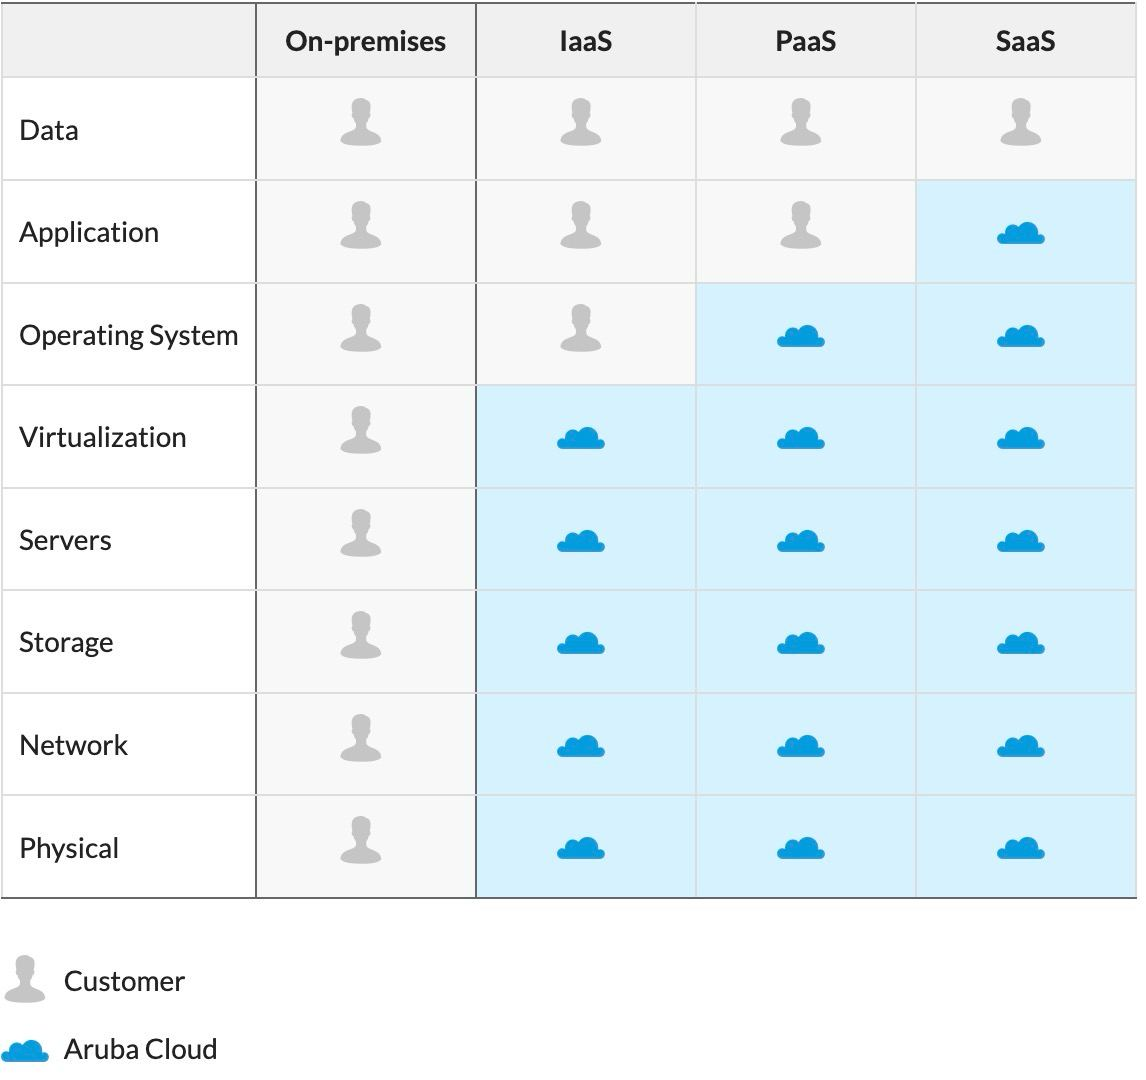
\includegraphics[width=1\textwidth]{aruba-shared-responsibility-model.png}
        \caption{Aruba Shared Responsibility Model}
    \end{figure}

    \newpage
    \textbf{AWS Shared Responsibility Model}
    \href{https://aws.amazon.com/it/compliance/shared-responsibility-model/}{AWS Shared Responsibility Model}\footcite{site:aws-shared-responsibility-model} is a model that defines the responsibilities of AWS and the customer for security, in the image below the shared responsibility model, with a clear division of responsibilitie between the provider and the customer, is shown.\\
    \begin{figure}[htbp]
        \centering
        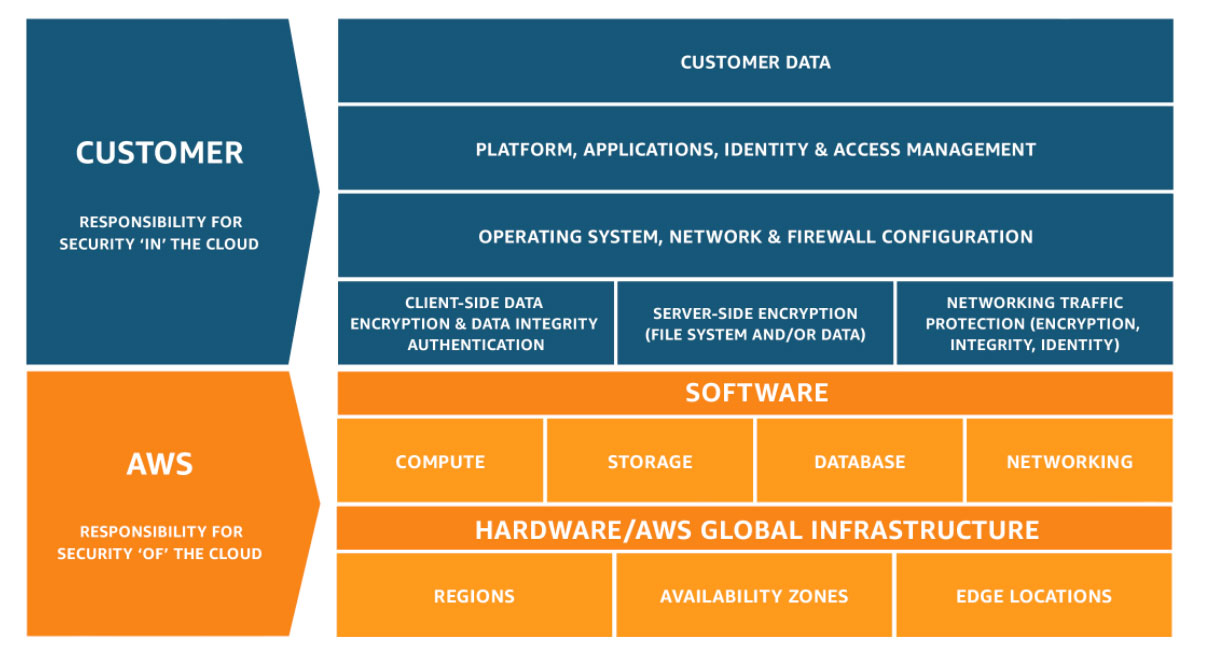
\includegraphics[width=1\textwidth]{aws-shared-responsibility.png}
        \caption{AWS Shared Responsibility Model}
    \end{figure}

    \newpage
    \textbf{Azure Shared Responsibility Model}
    \href{https://learn.microsoft.com/en-us/azure/security/fundamentals/shared-responsibility}{Azure Shared Responsibility Model}\footcite{site:azure-shared-responsibility-model} also defines the responsibilities of Azure and the customer for security, in the image below the shared responsibility model is shown with the main focus of dividing the responsibilities of the customer and the provider in case of the usage of \textit{Infrastructure as a Service} (IaaS), \textit{Platform as a Service} (PaaS) services and \textit{Software as a Service} (SaaS) services.\\
    
    \begin{figure}[htbp]
        \centering
        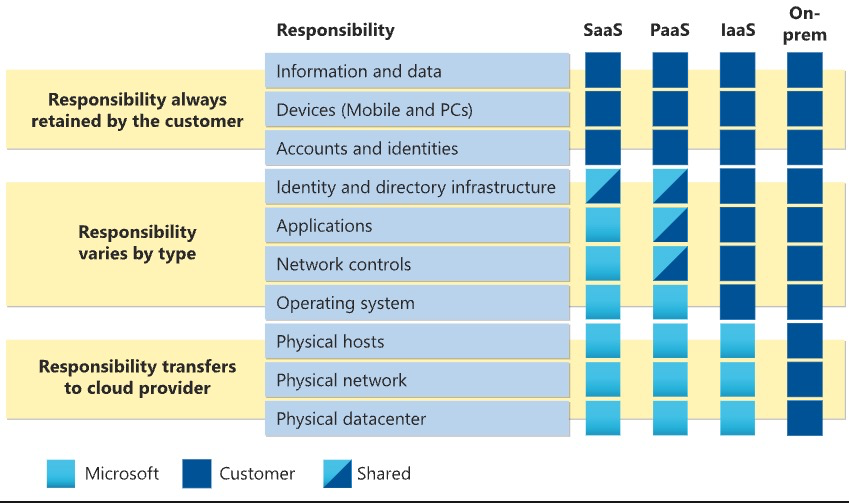
\includegraphics[width=1\textwidth]{azure-shared-responsibility.png}
        \caption{Azure Shared Responsibility Model}
    \end{figure}

\subsection{Scalability}
The system must be able to scale horizontally by adding more instances of the same service and must be able to scale vertically by increasing the resources of the service. The system must be able to automatically scale based on the load of the system.
Stress tests must be performed to verify the scalability of the system.\\

